
    \begin{abstract_online}{Water-Mediated Curvature Change in Graphene by Single-Walled Carbon Nanotube: A Molecular Dynamics Study}{%
        \underline{H. M. Gade}$^{1}$, P. P. Wanjari$^{2}$, S. V. V. Velpuri$^{2}$}{%
        }{%
        $^1$ Department of Chemical Engineering, IIT Bombay, India\newline{}$^2$ Department of Chemical Engineering, Visvesvaraya National Institute of Technology, Nagpur, India}
    Novel nanostructured materials possessing new architectural segments can be synthesized using the various combinations of graphenes and carbon nanotubes (CNT) that can result into the generation of enhanced physico-chemical properties within the hybrids. Comprehending the various physical processes involved in the creation of these new segments is crucial for designing an optimized nanomaterial for a specific purpose. In this work we report induced folding in a graphene sheet resulting from the physical interactions between a water-mediated graphene and a CNT. Owing to robust binding interactions between the CNT and a compatible graphene sheet, the latter forms a second domed layer around the former culminating in a structure equivalent to a double-walled CNT. The induced curvature change in graphene by CNT was found to have strong dependencies upon their relative physical dimensions. For example, CNT possessing extreme small diameters are unable to induce any significant curvature changes in longer graphene sheets. The potential-of-mean force (PMF) between our reference graphene and CNT in water suggests a favorable binding interaction of −14.5 kcal mol-1. The breakdown of PMF into direct graphene-nanotube interactions and water-mediated interactions reveals huge reduction in the strongly attractive binding interactions between graphene and CNT by the water molecules. \begin{center}  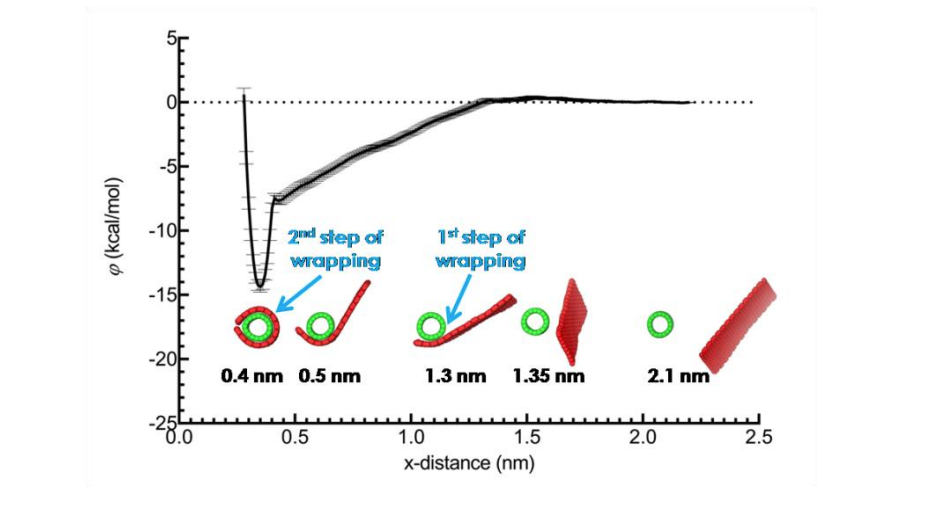
\includegraphics[width=0.8\linewidth]{abstracts/txt/figures/hrushi.png}  \caption{Potential-of-mean force for pulling center of mass of graphene from the bulk water on the outer surface of CNT along the x-axis.}  \end{center}  
    
        \textbf{References} \newline{}[1] Gade H.M. et al., Physical Chemistry Chemical Physics, 20 (34) 2018, 22359-22367.\newline{}[2] Athawale M.V. et al., Journal of Chemical Physics, 131(11), 2009, 09B615.\newline{}[3] Patra N. et al., ACS Nano, 5, 2011, 1798-1804\newline{}[4] Makowski et al., Journal of Physical Chemistry B,114, 2010, 993-1003 
    \end{abstract_online}
    